\documentclass{article}
\usepackage{amsmath}
\usepackage{graphicx}
\usepackage{float}
\usepackage{hyperref}
\usepackage{fancyhdr}
\usepackage[a4paper, margin=1in]{geometry}
\usepackage{xeCJK}
\usepackage{fontspec}

\setCJKmainfont{SimSun} % 设置中文字体

\title{OpenMV开发板实验报告}
\author{杜佳颖 2021533037}
\date{\today}

\pagestyle{fancy}
\fancyhead{}
\fancyfoot{}
\fancyfoot[R]{\thepage}

\begin{document}

\maketitle

\section{引言}
由于本次项目第二个任务开始后我并不在学校,我使用远程USB软件进行本次项目开发。此次实验使用OpenMV H7开发板,完成了三个任务:
\begin{enumerate}
    \item 使用三种不同颜色的灯闪烁。
    \item 检测并圈出蓝色色块。
    \item 检测蓝色色块并用舵机跟随,使其中心点一直保持在画面中心。
\end{enumerate}

OpenMV H7是一款功能强大的微控制器板,专为图像处理应用设计,采用ARM Cortex-M7处理器,能够实时执行计算机视觉任务。通过本次实验,展示了OpenMV H7开发板在图像处理和舵机控制方面的实际应用。

\section{设备}
\begin{itemize}
    \item OpenMV H7开发板
    \item 三种颜色的LED
    \item 舵机
    \item 蓝色物体(用于颜色跟踪)
\end{itemize}

\section{任务1:使用三种不同颜色的灯闪烁}
\subsection{实现方法}
通过OpenMV H7开发板上的\texttt{pyb}模块控制LED的亮灭。我发现这一任务的实现相对简单,主要是通过控制微控制器的GPIO引脚使LED亮灭。每个LED按顺序亮起1秒后熄灭1秒,循环进行。初次尝试时遇到了一些延时问题,通过调整代码中的延时函数解决了这一问题。

\subsection{原理}
LED的亮灭通过将GPIO引脚设置为高电平实现,电流流经LED使其发光。使用延迟函数引入延迟以实现闪烁效果。这一过程让我更好地理解了基本的GPIO控制和时间延迟在实际应用中的效果。

\begin{figure}[H]
    \centering
    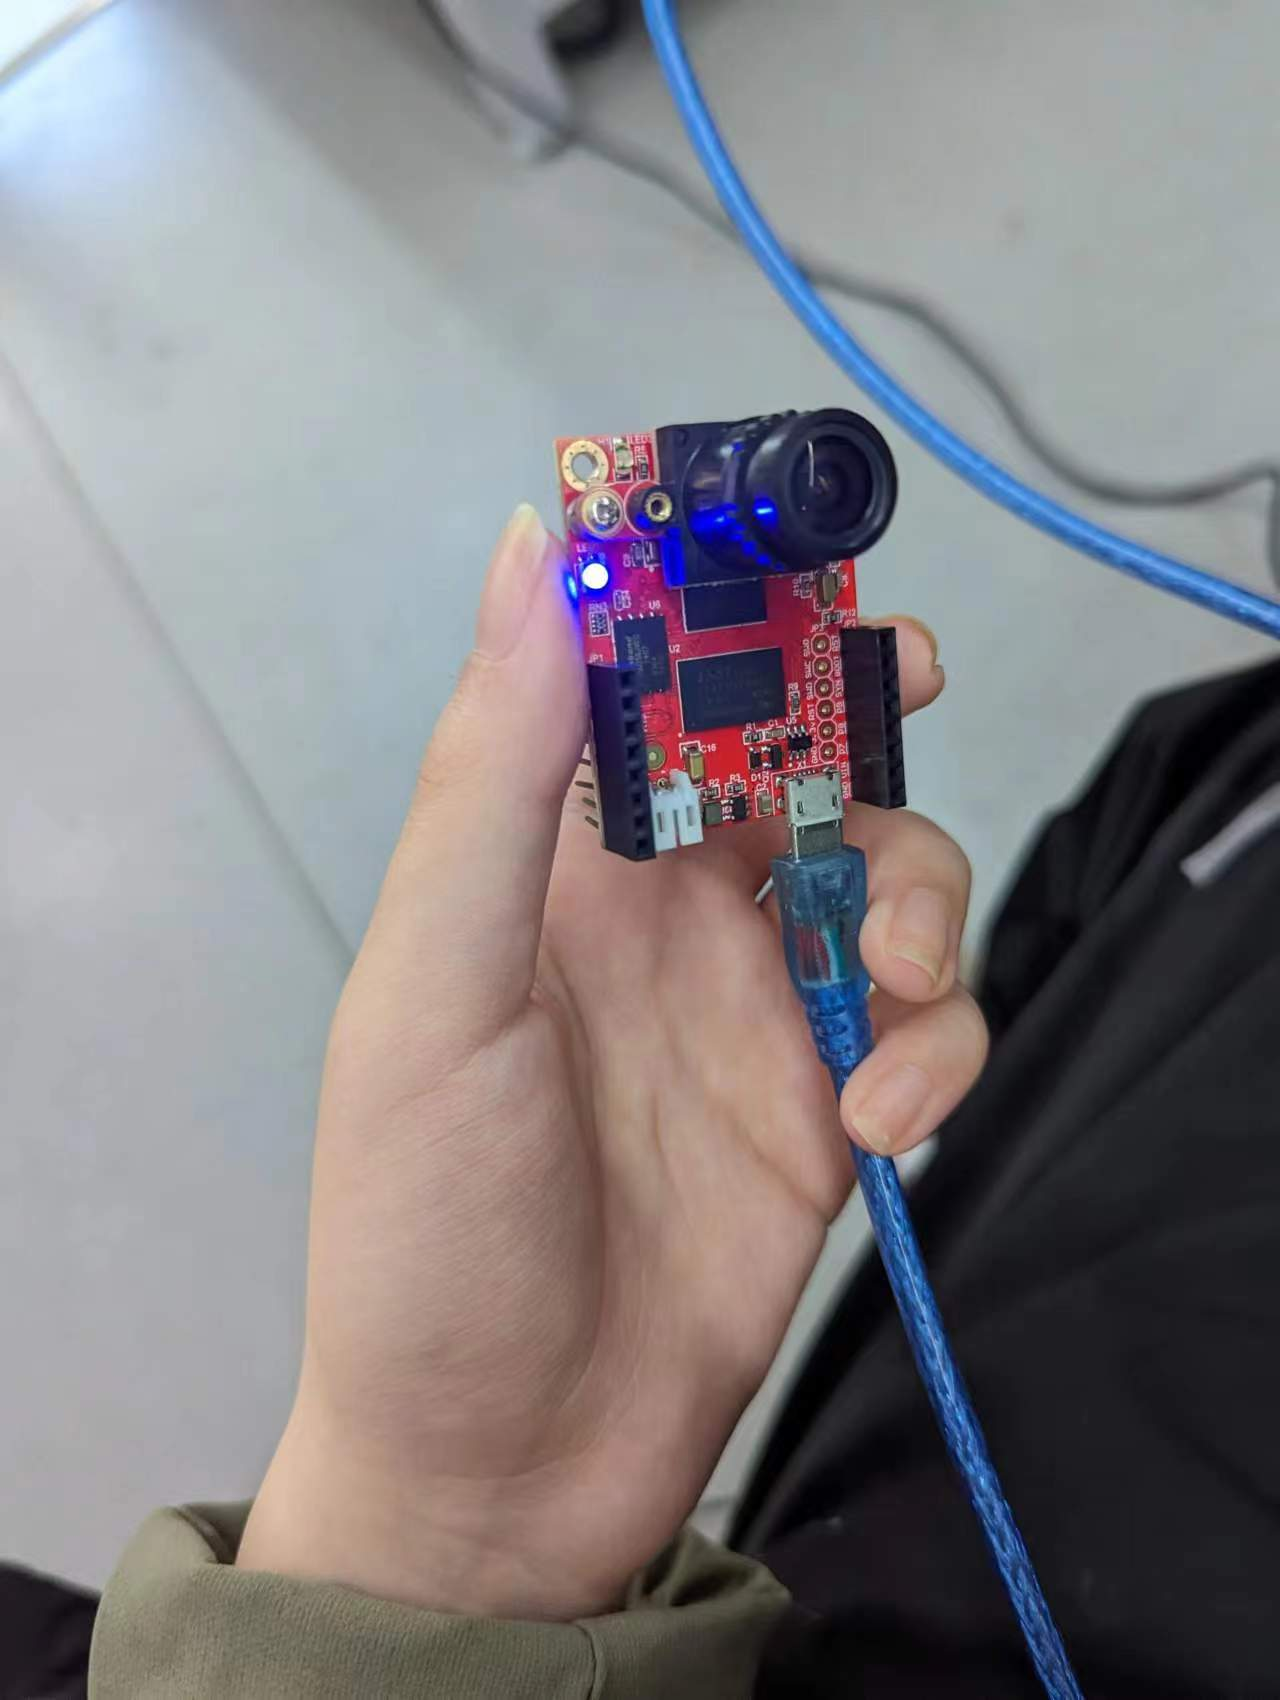
\includegraphics[width=300pt]{./LED.jpg}
    \caption{OpenMV H7开发板上的LED设置}
\end{figure}

\section{任务2:检测并圈出蓝色色块}
\subsection{实现方法}
在这一任务中,我们利用OpenMV H7的图像处理功能,检测图像中的蓝色色块并在其周围画圈。设置颜色跟踪阈值后,摄像头捕捉图像,识别出符合蓝色阈值的区域,并在这些区域的中心点画圈和十字。调试时,我通过多次调整颜色阈值,最终找到了最佳设置,使得检测更加准确。

\subsection{原理}
颜色检测基于LAB颜色空间,将亮度与颜色分量分离,这使得在不同光照条件下分割特定颜色更加容易。通过\texttt{find\_blobs}方法识别图像中匹配颜色阈值的区域,并使用\texttt{draw\_circle}方法在这些区域周围画圈。在实际操作中,我体会到了图像处理的复杂性以及调试过程的重要性。
\section{任务3:用舵机跟随蓝色色块}
\subsection{实现方法}
为了使蓝色色块保持在画面中心,我们使用了两个舵机来调整相机的方向。通过计算检测到的色块中心与屏幕中心的偏移量,调整舵机角度,使色块中心保持在画面中心。这一任务的实现让我更加了解了反馈控制系统的原理,并且在调试过程中学会了如何调整舵机的响应速度和精度。

由于远程开发的限制,我本人无法直接观察舵机的运动,因此我通过调整舵机角度和颜色阈值,根据组员的观察情况,不断测试和调试,最终实现了舵机跟踪蓝色色块的功能。

\subsection{原理}
通过计算检测到的色块中心与屏幕中心的偏移量,调整舵机角度,使色块中心保持在画面中心。这是一种基本的反馈控制,通过不断调整舵机角度来最小化位置误差。在调试过程中,我深刻体会到了实时控制的重要性以及系统响应速度对控制效果的影响。

\section{结论}
此次实验成功演示了OpenMV H7开发板在控制LED闪烁、检测颜色并绘制图形、以及舵机跟踪方面的应用。在整个开发过程中,我不仅熟悉了OpenMV H7的硬件和软件特性,还体验了远程开发的挑战和乐趣。每个任务的完成都让我对嵌入式系统和图像处理有了更深的理解。

利用STM32H7处理器的高性能,OpenMV H7能够处理复杂的任务,包括高速图像处理和精确的电机控制,使其成为机器人和自动化项目的理想平台。这次实验经历也为我未来的开发工作提供了宝贵的经验。

\end{document}
